\documentclass[12pt,beamer]{beamer}
\usepackage{graphicx}
\usepackage{multicol}
\usepackage{adjustbox} %table 的缩放
\useoutertheme[links=true,sections=false]{progressbarjma}

\usecolortheme{whale}
\setbeamertemplate{blocks}[rounded][shadow=true]
\setbeamertemplate{theorems}[numbered]
\setbeamertemplate{items}[ball] 
\setbeamertemplate{sections/subsections in toc}[ball]
\setbeamercolor{item projected}{bg=blue!50} 


\usepackage[round]{natbib}

\def\suppressnavigationsymbols{%
\setbeamertemplate{navigation symbols}{}}

% listing
\usepackage{caption}
\setbeamertemplate{caption}[numbered]
\usepackage{color}
\usepackage{listings} 


\def\restorenavigationsymbols{%
    \setbeamertemplate{navigation symbols}{%
        \insertslidenavigationsymbol
        \insertframenavigationsymbol
        \hskip1.5pt
        \insertindexnavigationsymbol
        \insertdocnavigationsymbol
        \insertbackfindforwardnavigationsymbol
    }%
}

% The following is needed, otherwise LaTeX will complain 
% when typesetting the bibliography...
\def\newblock{\hskip .11em plus .33em minus .07em}

%\renewcommand{\normalsize}{\fontsize{10pt}{\baselineskip}\selectfont}
\usefonttheme{professionalfonts}
\usefonttheme{structurebold}
\usefonttheme{structureitalicserif}
\usefonttheme{structuresmallcapsserif}
\title[]{Model Based Formal Design for MVB System}
\author{Ji Qi, Kueiming Lo}

\institute[LSE] 
{
    School of Software, Tsinghua University, \\
    Beijing 100084, China
}

\date{27 July 2017}

% Delete this, if you do not want the table of contents to pop up at
% the beginning of each subsection:

\AtBeginSection
{
	\begin{frame}		
		\frametitle{Contents}
		\begin{multicols}{2}
			\small{\tableofcontents[currentsection]}
		\end{multicols}
	\end{frame}
}


\lstset{
	language=VHDL,
	numbers=left,
	numberstyle=\small,
	numbersep=5pt,                   % how far the line-numbers are from the code
	frame=tb,
	columns=fullflexible,
	showstringspaces=false,
	xleftmargin=2em,
	xrightmargin=2em, 
	aboveskip=1em
}

\usepackage{caption}
\captionsetup{font={scriptsize}} 


\begin{document}



\suppressnavigationsymbols

\begin{frame}[plain]
    \titlepage
\end{frame}

\restorenavigationsymbols


\begin{frame}{Outline}
    \tableofcontents[hideallsubsections]
\end{frame}

\section{Background}

\subsection{Background}


\begin{frame}
	\frametitle{Background}
	There is a growing demand of computing resources due to the development of artificial intelligence.
	
	CPU and GPU may not fulfill the requirements.
	
	FPGA and ASIC are widely used to accelerate machine learning algorithms, IoT, and other data intensive tasks.


	\vspace{10pt}	
	\begin{columns}[T]
		\column{0.4\textwidth}
		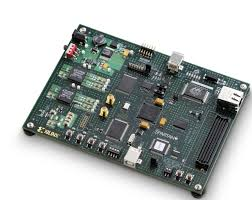
\includegraphics[width=\textwidth]{pic/circuit1.jpeg}
		\column{0.3\textwidth}
		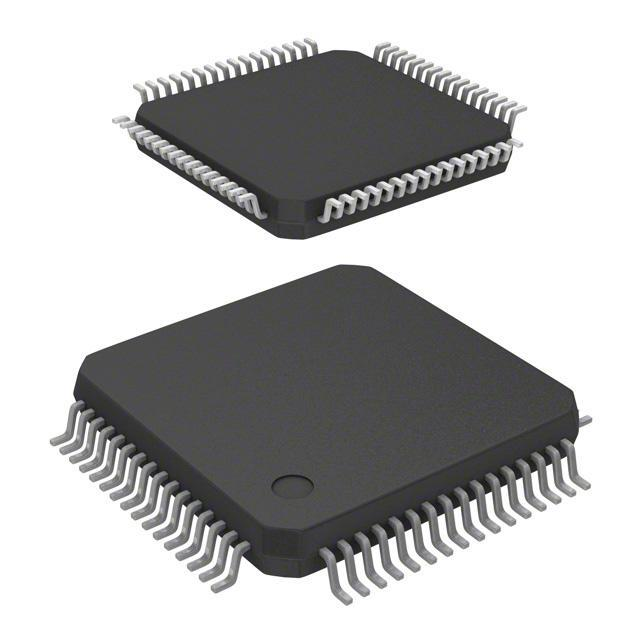
\includegraphics[width=\textwidth]{pic/circuit2.jpg}
	\end{columns}
	
\end{frame}

\subsection{Bottom-up methodology}

\begin{frame}[c]
	In traditional circuit development, the bottom-up methodology was first used. The design flow is based on basic electronic components, continue to function block components, and finally specify a whole system.
	
	\frametitle{Bottom-up methodology}
	\begin{block}{Weakness}
	\begin{itemize}
		\item Hardware design must be understood by the designer.
		\item Developers can only test the design after getting the circuit.
		\item Hard to develop and maintain.
		\item ...
	\end{itemize}
	\end{block}
\end{frame}

\subsection{Top-down methodology}
\begin{frame}[c]
	\frametitle{Top-down methodology}
		\begin{columns}[T]
			\column{0.5\textwidth}
			\begin{itemize}
			\setlength{\itemsep}{5pt}
			\item HDLs are used to describe the system behavior.
			\item The behavior of the system can be verified before getting the real hardware.
			\item Synthesis tools can translate the design into hardware directly.
			\item Not good enough.
			\end{itemize}

			\column{0.5\textwidth}
			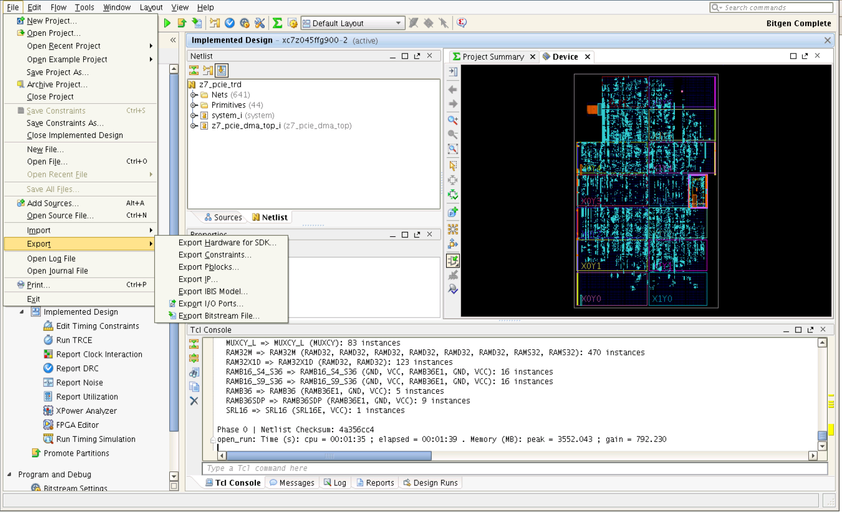
\includegraphics[width=\textwidth]{pic/xilinx.png}\\
			Getting hardware directly by synthesis tools(Xilinx ISE).
		\end{columns}
\end{frame}


\subsection{Formal modeling method}

\begin{frame}
	\frametitle{Formal modeling method}
	\begin{center}
	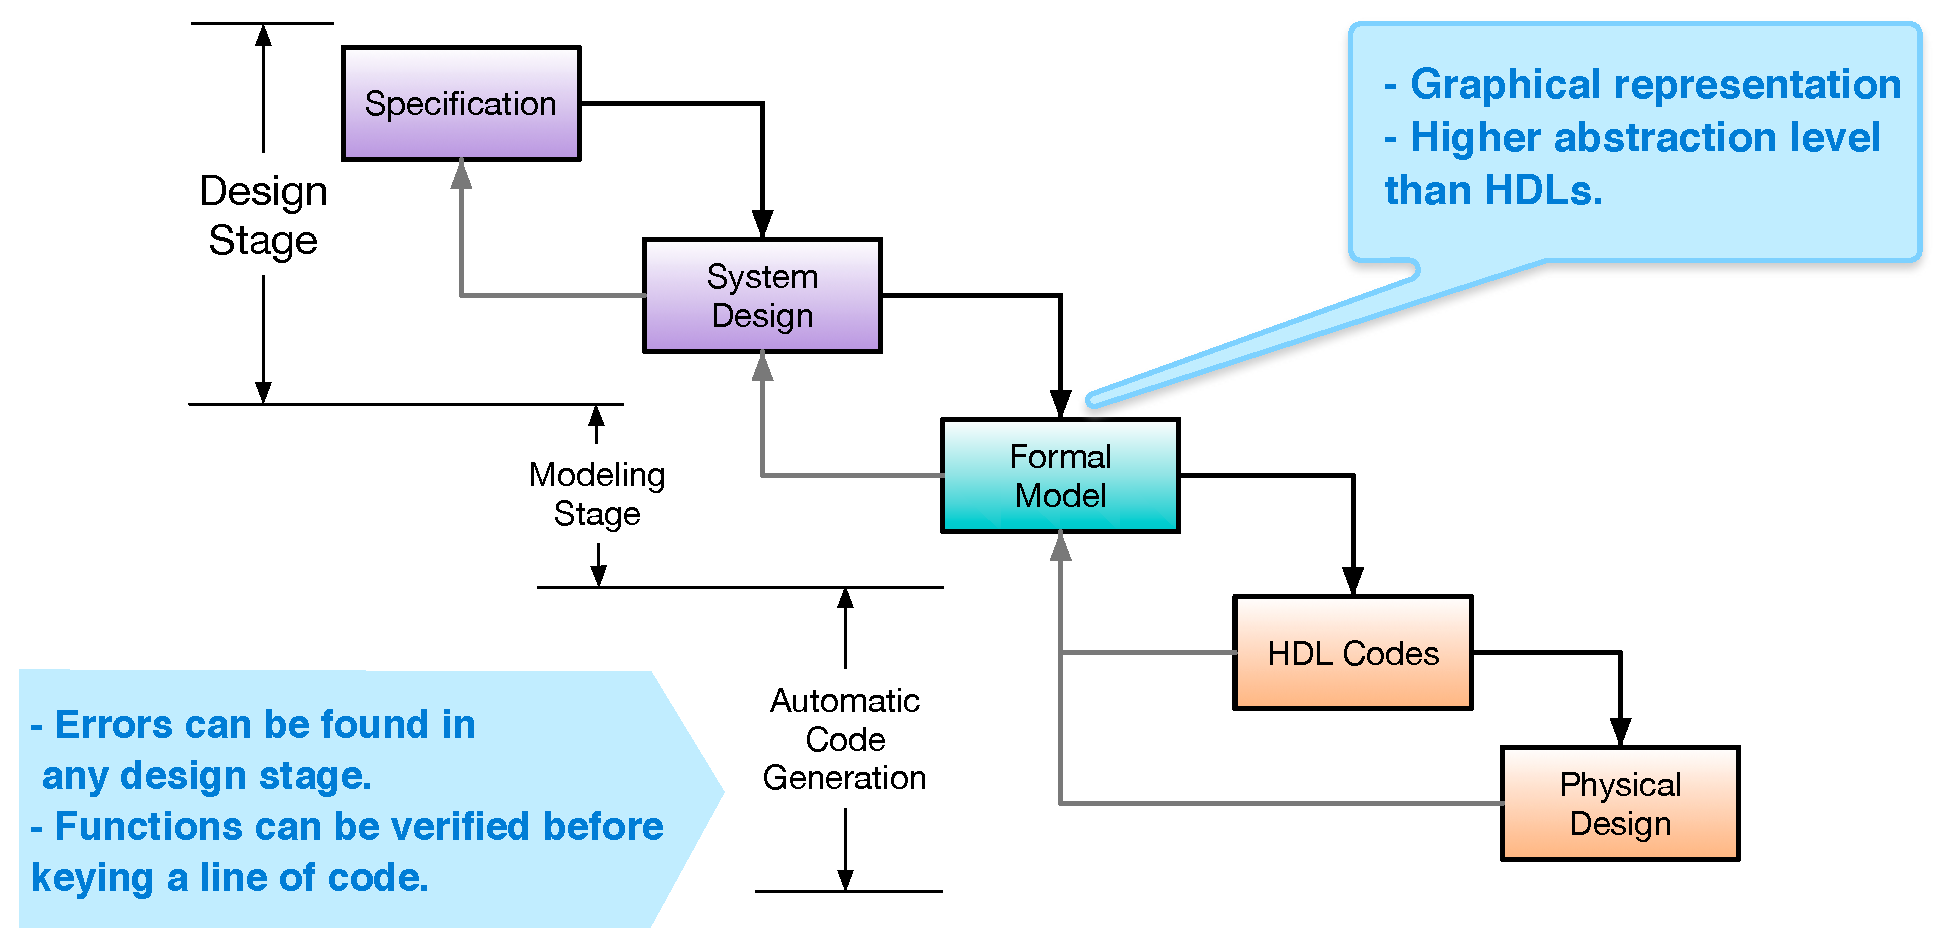
\includegraphics[width=\textwidth]{pic/Development_Process.pdf}
	\end{center}
	%A higher level abstraction than VHDL.\\
	%The later bugs are found, the higher the cost of repair.\\
	%Build prototypes rapidly and verify the system design before keying a line of HDL code. 
\end{frame}



\begin{frame}[c]{Multifunction Vehicle Bus}

Multifunction Vehicle Bus (MVB) is a high-dependency field bus designed for railroad vehicle control systems.

Master-Slave architecture:
\begin{center}
\includegraphics[width=0.7\textwidth]{pic/mvb.pdf}
\end{center}
%\begin{enumerate}
%	\item Only one master device.
%	\item Master device broadcasts the main frame with $Addr$ periodically.
%	\item Slave devices whose address correspond with $Addr$ should response to master device by slave frame.
%	\item Qualified devices would be master device in turn through mastership transfer.
%\end{enumerate}
\end{frame}

\begin{frame}{Multifunction Vehicle Bus}

\begin{itemize}
	\setlength{\itemsep}{10pt}
	\item MVB has been developed with HDLs(top-down methodology)
	\item Few investigations have been published regarding MVB development with formal modeling methods. 
	\item This is the motivation for us to develop MVB with this novel method.
\end{itemize}

\vspace{1em}
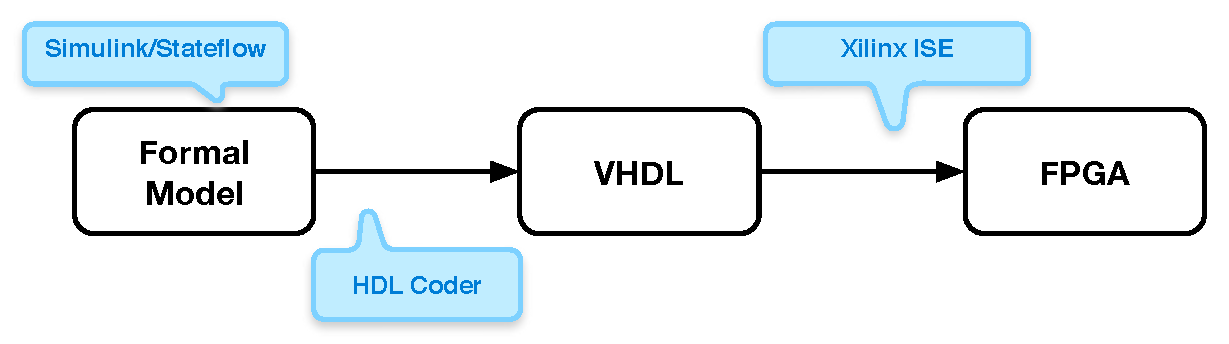
\includegraphics[width=\textwidth]{pic/Study_Process.pdf}
\end{frame}

\section{Experiment process}


\subsection{Formal modeling}

\begin{frame}
\frametitle{Device design}
\begin{center}
	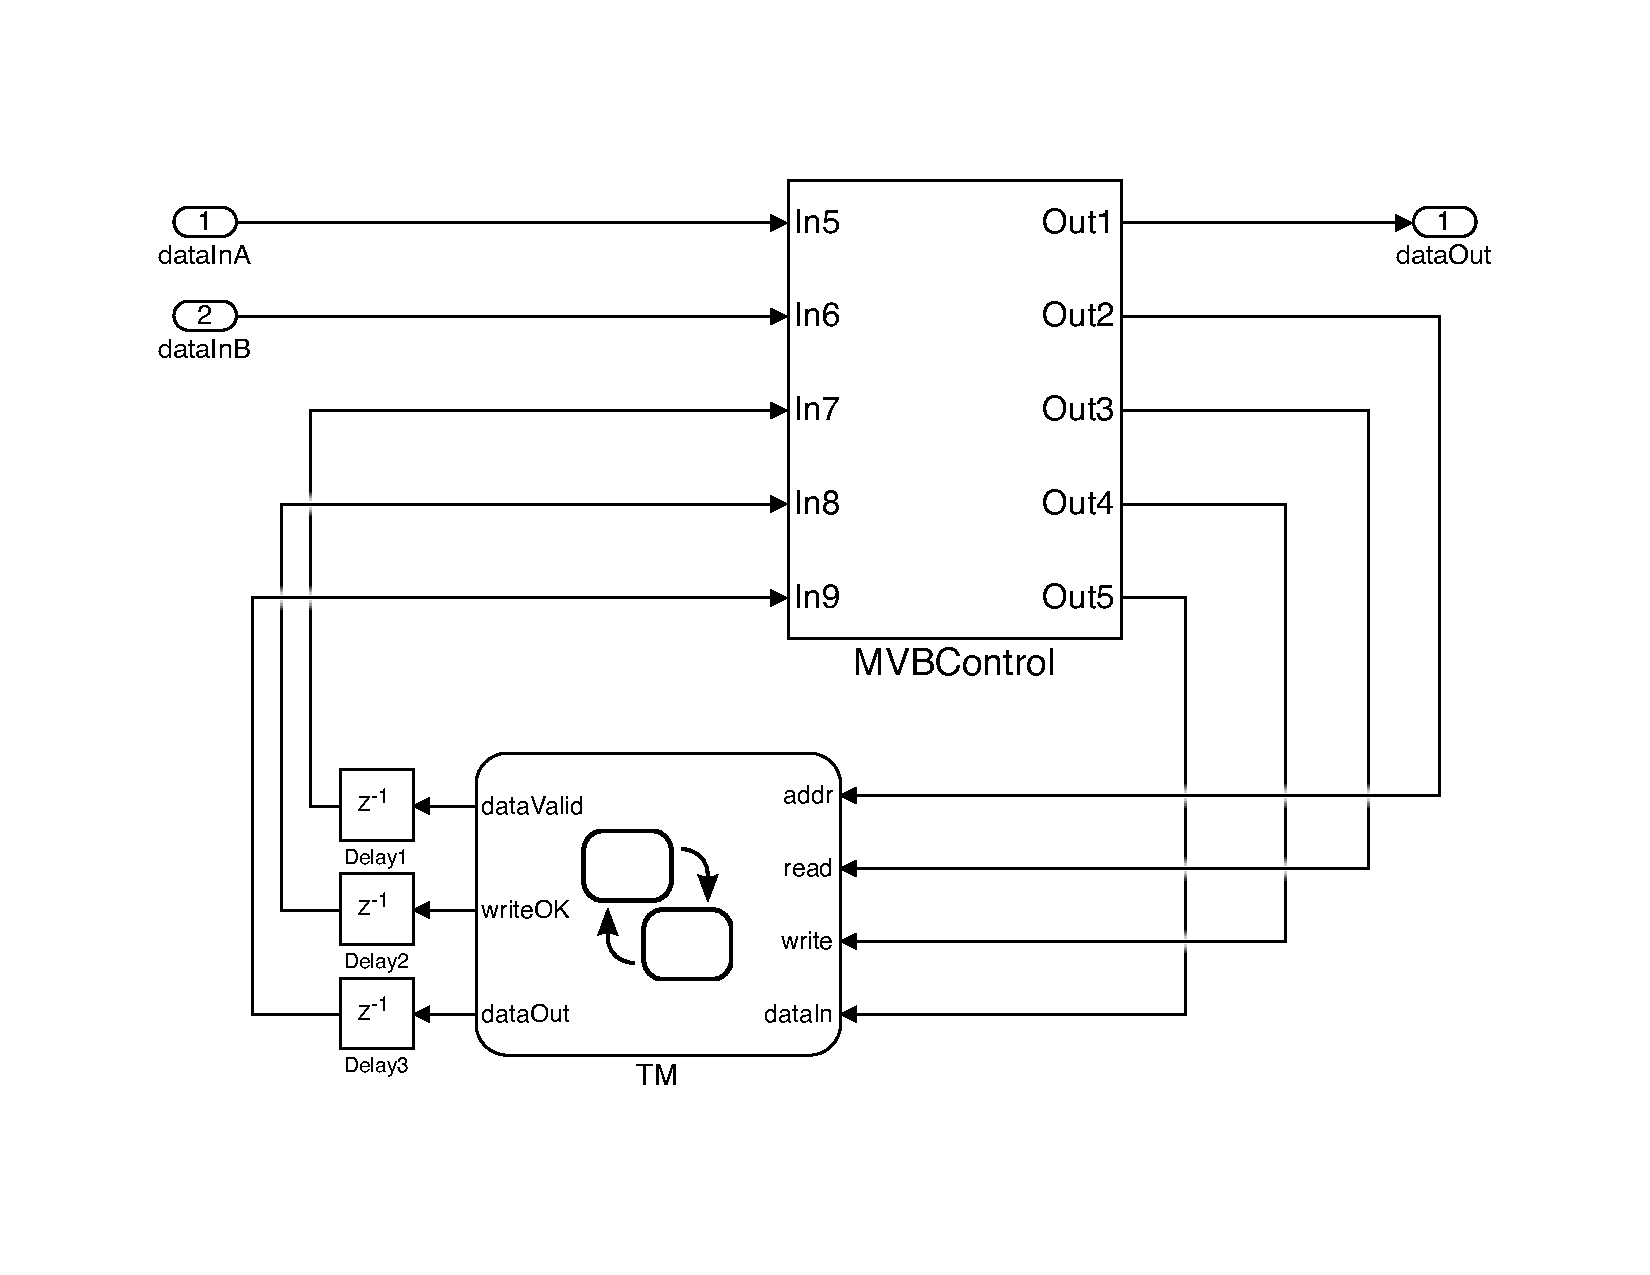
\includegraphics[width=0.8\textwidth]{pic/Device_design.pdf}
\end{center}
\end{frame}

\begin{frame}
\frametitle{MVB Controller}
\begin{center}
	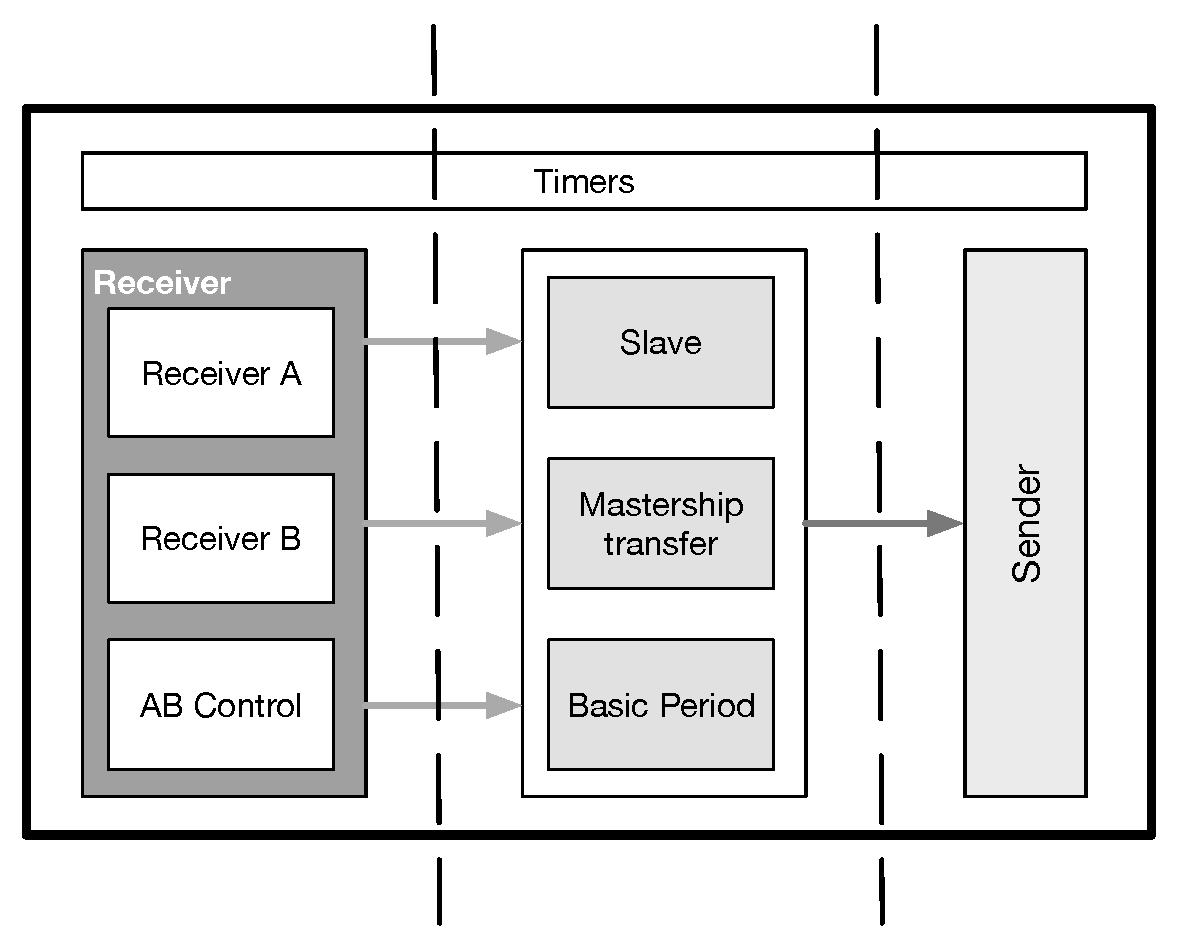
\includegraphics[width=0.8\textwidth]{pic/Module_Division.pdf}	
\end{center}
\end{frame}

\begin{frame}{Sender module}
\begin{columns}
	\begin{column}{.25\textwidth}
	\begin{figure}
	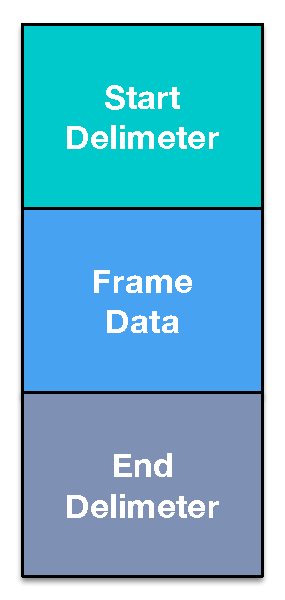
\includegraphics[width=\textwidth]{pic/Frame.pdf}
	\end{figure}
	\end{column}
	\begin{column}{.8\textwidth}
	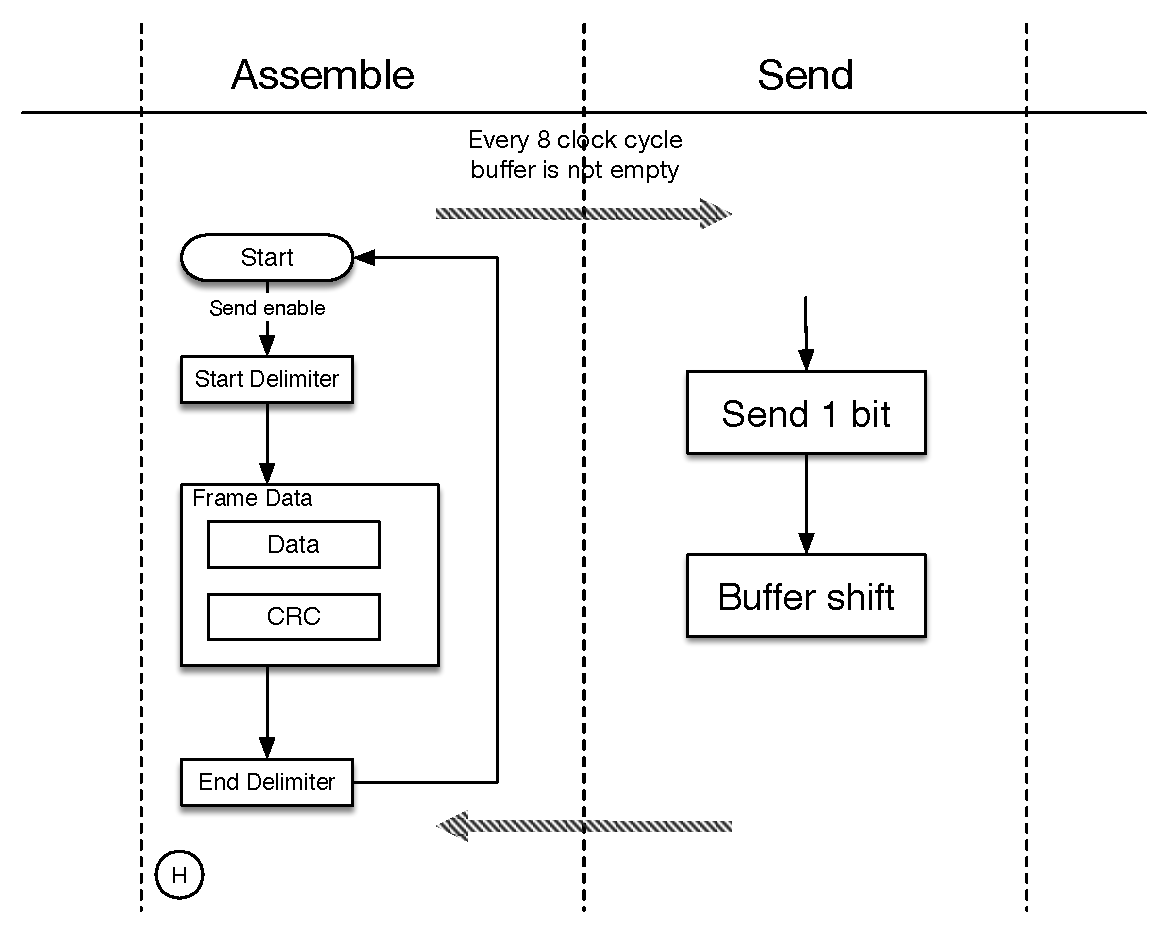
\includegraphics[width=\textwidth]{pic/sender.pdf}
	\end{column}
\end{columns}

\end{frame}


\begin{frame}
\frametitle{Receiver module}
\centering
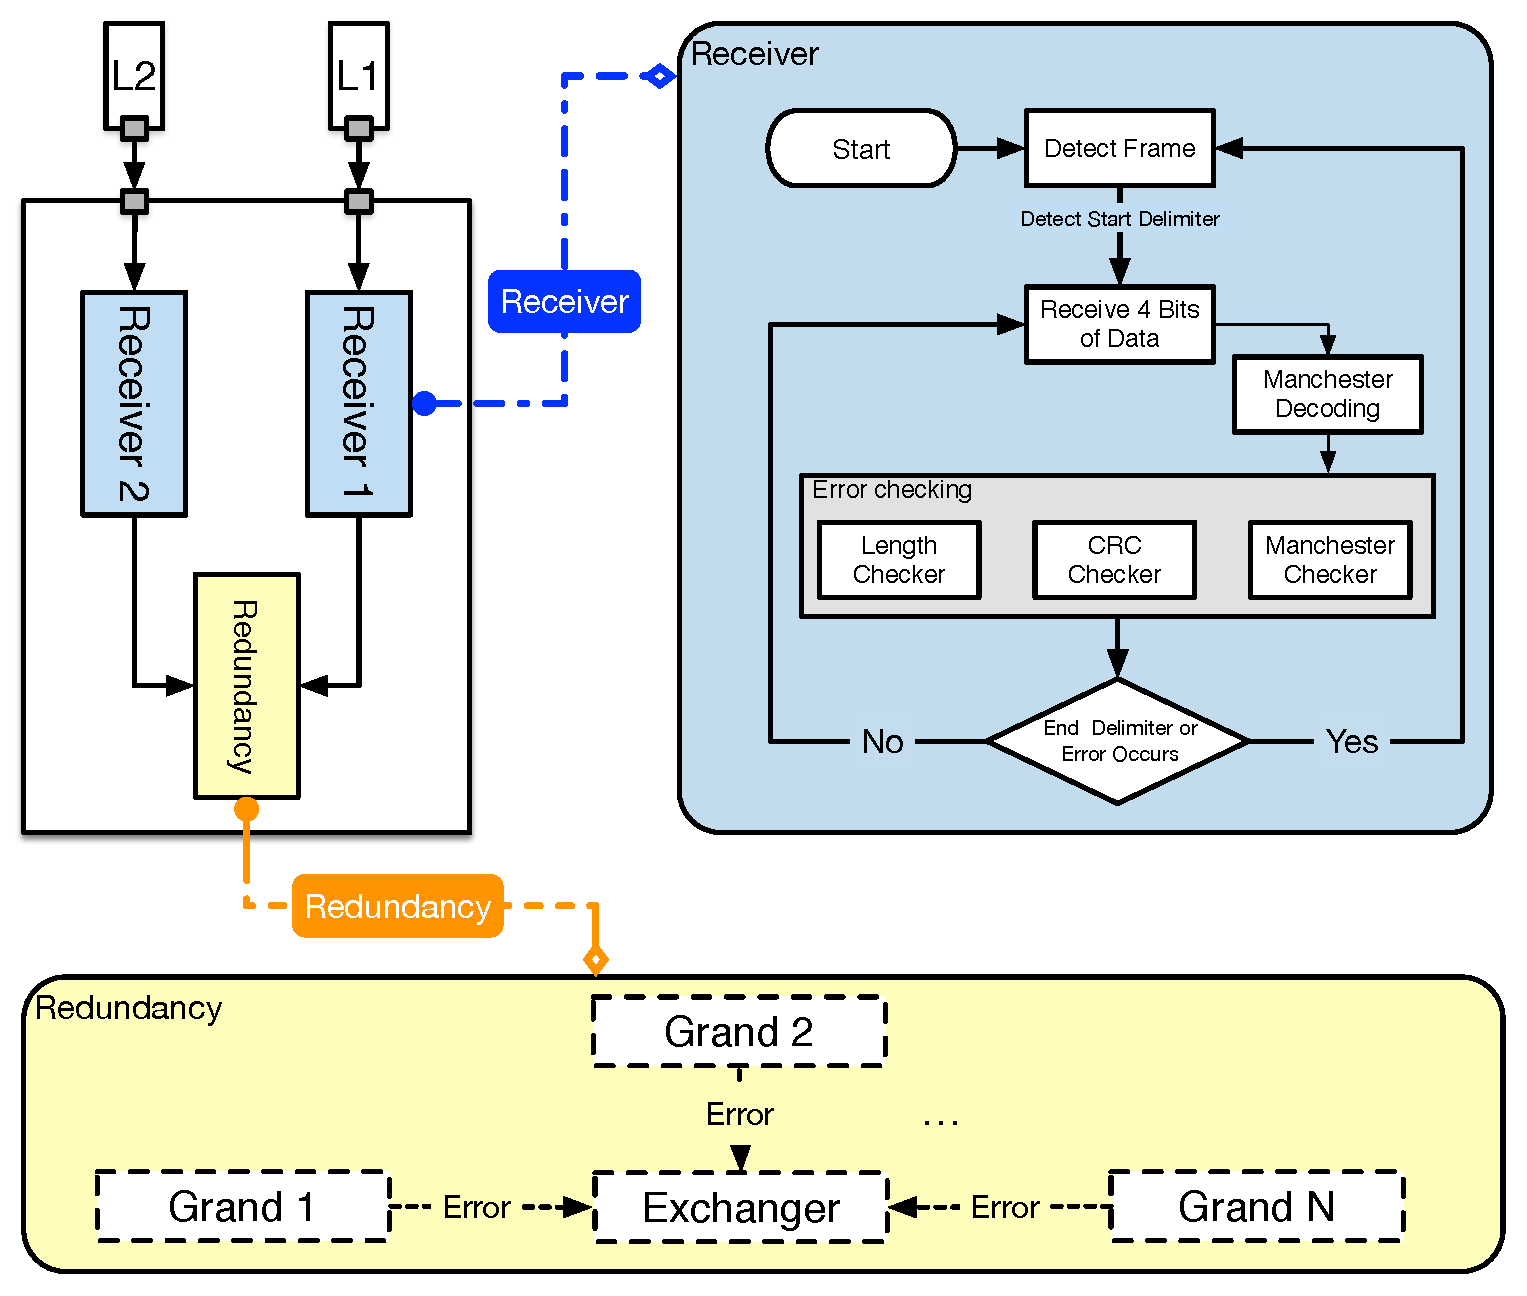
\includegraphics[width=0.8\textwidth]{pic/Receiver.pdf}
\end{frame}

\begin{frame}
	\frametitle{Redundancy module}
		\begin{enumerate}
			\setlength{\itemsep}{20pt}
			\item If no valid frame has been received from the Trusted\_Line for T\_switchover since the end of the last valid Master Frame or the last switchover;
			\item If the receiver of the Observed\_Line detects a valid frame and the receiver of the Trusted\_Line detects no valid frame within T\_skew\_r;
			\item If a valid frame has been received over the Trusted\_Line, but the check sequence or the frame length is mistaken.
		\end{enumerate}
\end{frame}




%\begin{frame}[fragile, shrink]{Manchester decoding}
%\begin{lstlisting}[caption={Manchester Decoding}]
%function Manchester_Decode
%    if (data(1:4) = [1 0 1 0]) recv=recv*4;
%    elseif (data(1:4) = [1 0 0 1]) recv=recv*4+1;
%    elseif (data(1:4) = [0 1 1 0]) recv=recv*4+2;
%    elseif (data(1:4) = [0 1 0 1]) recv=recv*4+3;
%    elseif (data(1:4) = [1 1 1 1]) FrameEnd=true;
%    else Collision = true;
%    end
%end
%\end{lstlisting}
%\end{frame}



%\begin{frame}{Event arbitration}
%Event arbitration is designed to iterate all the events hanged by devices. Multiple devices can signal events at the same time. The master device must locate all of them.
%
%\begin{alertblock}{Important Definitions}
%\textbf{Addr:} In MVB system, each device is uniquely identified by its address Addr.
%
%\textbf{Event\_Device:} A device that signals event.
%
%\textbf{Group\_Addr:} Group\_Addr is a scope that contain several Addrs, i.e., $X0=\{00, 10\}$.
%\end{alertblock}
%\end{frame}
%
%\begin{frame}{Event arbitration tree}
%\center
%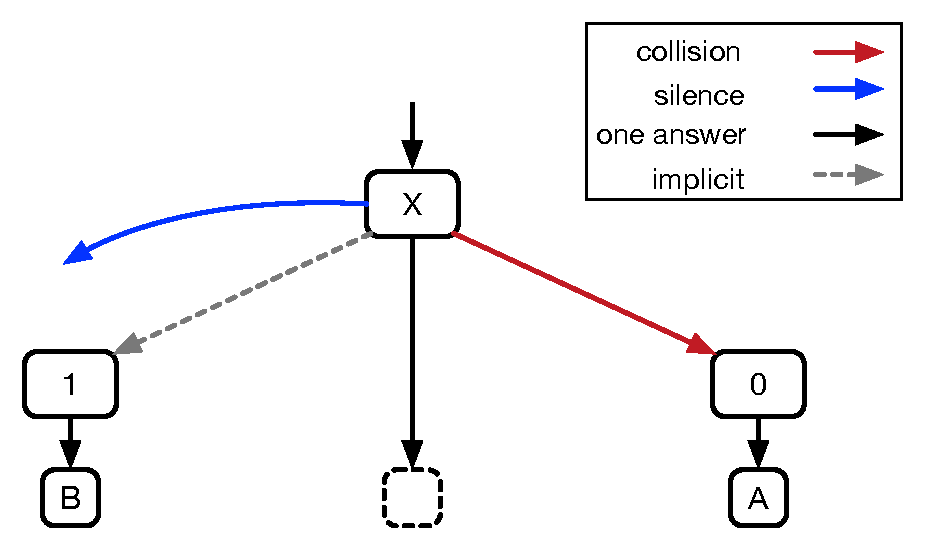
\includegraphics[width=\textwidth]{pic/SimpleTree.pdf}
%\end{frame}
%
%
%\begin{frame}{Event arbitration module}
%\center
%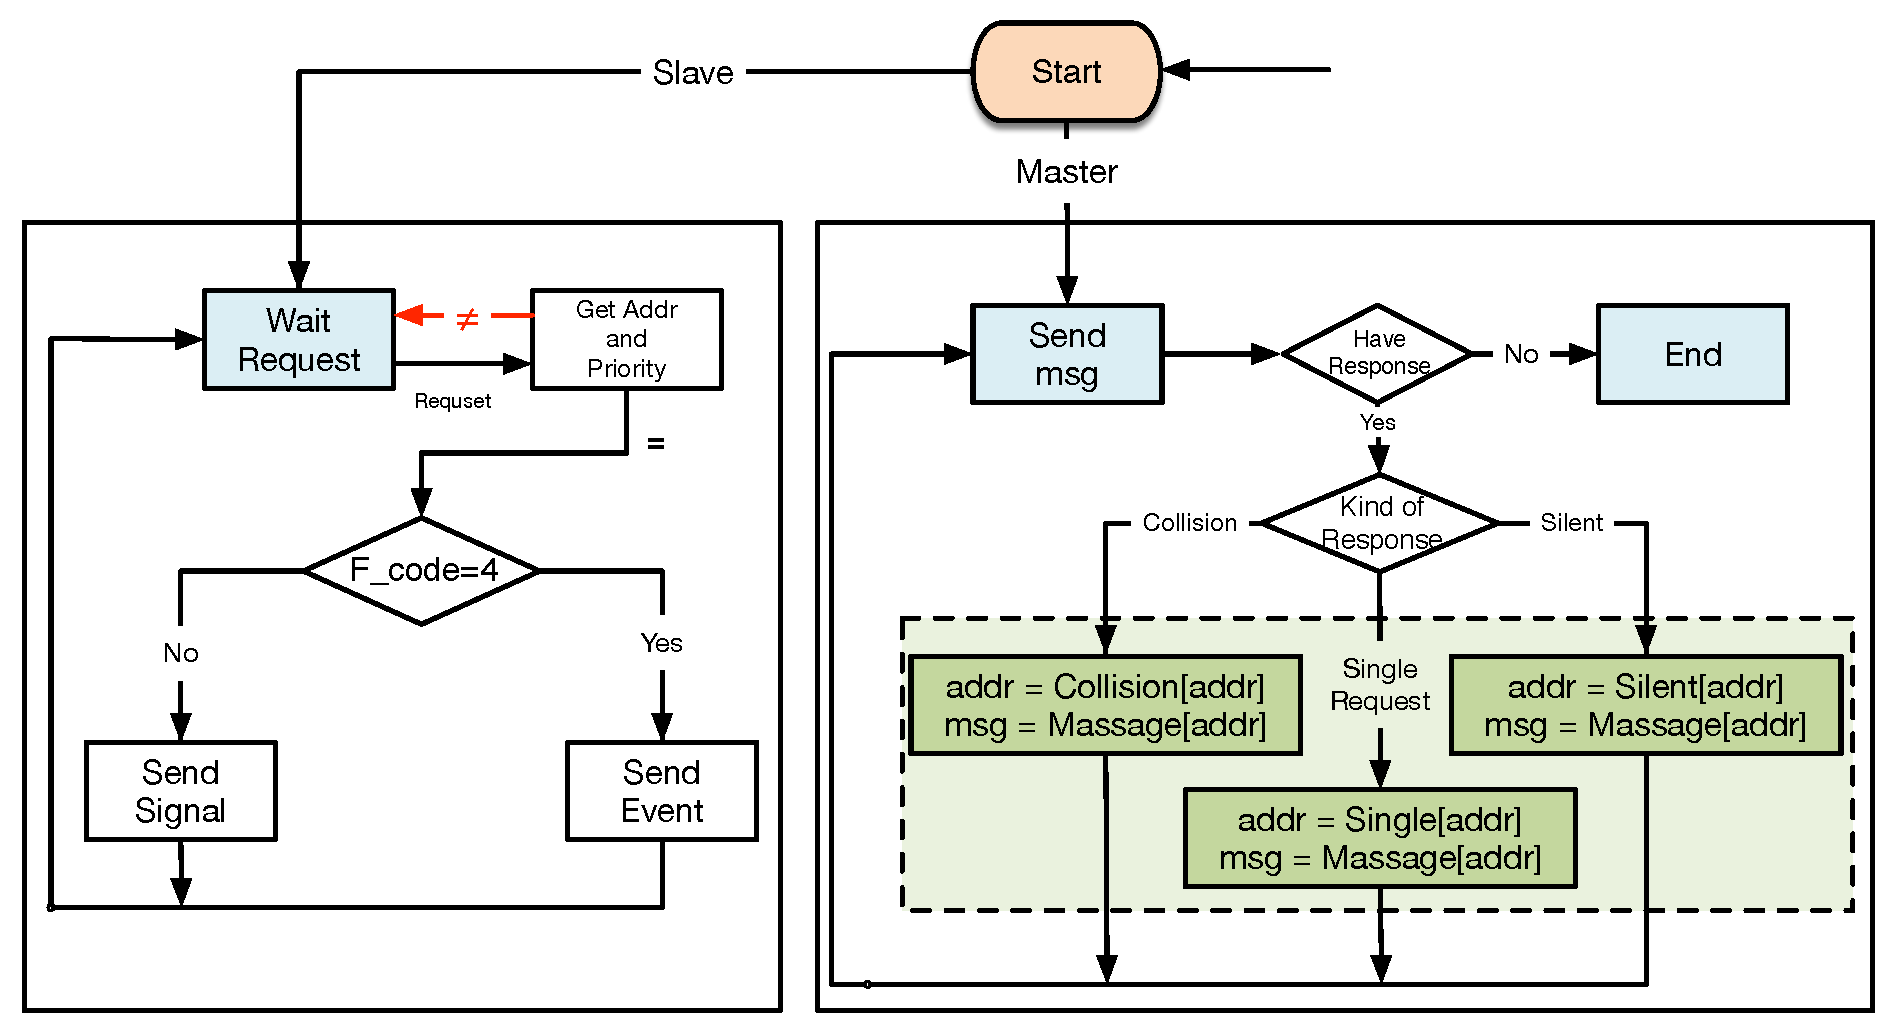
\includegraphics[width=\textwidth]{pic/EventArbitration.pdf}
%\end{frame}
%

\begin{frame}
\frametitle{System design}
\begin{columns}[c]
	\begin{column}{.4\textwidth}
		\begin{figure}
		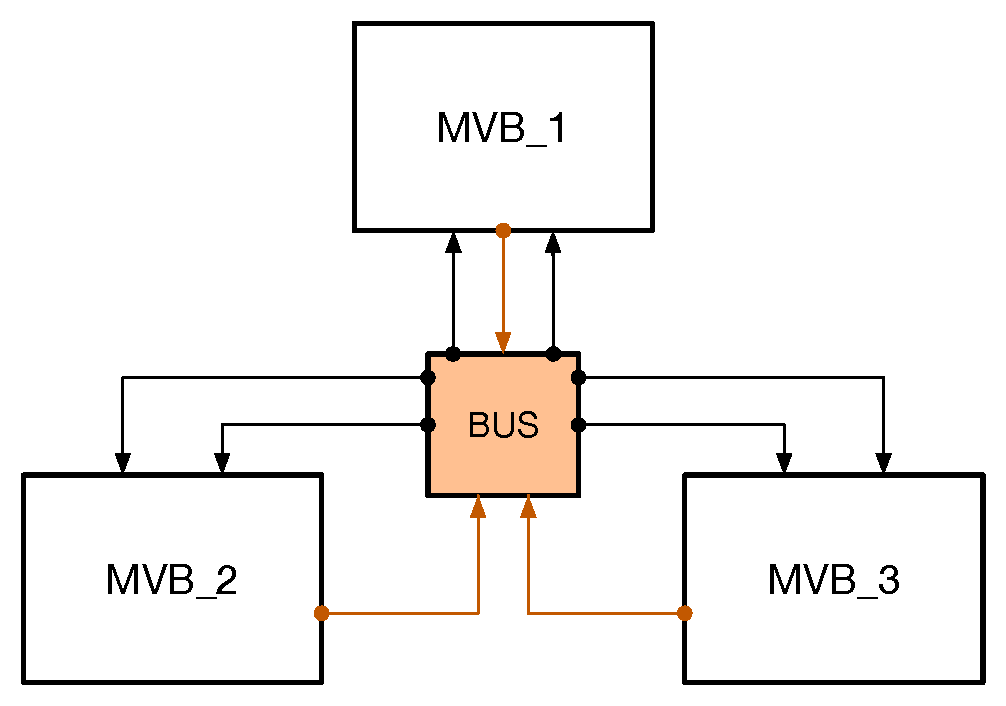
\includegraphics[width=\textwidth]{pic/Test.pdf}
		\caption{Testing environment}
		\end{figure}

		
	\end{column}
	
	\begin{column}{.5\textwidth}
		\begin{figure}
		\includegraphics[width=\textwidth]{pic/bus.pdf}
		\caption{Bus module}
		\end{figure}
	\end{column}
\end{columns}
\end{frame}

\begin{frame}
	\frametitle{Simulation}
	\begin{columns}
		\begin{column}{0.5\textwidth}
			\begin{figure}
			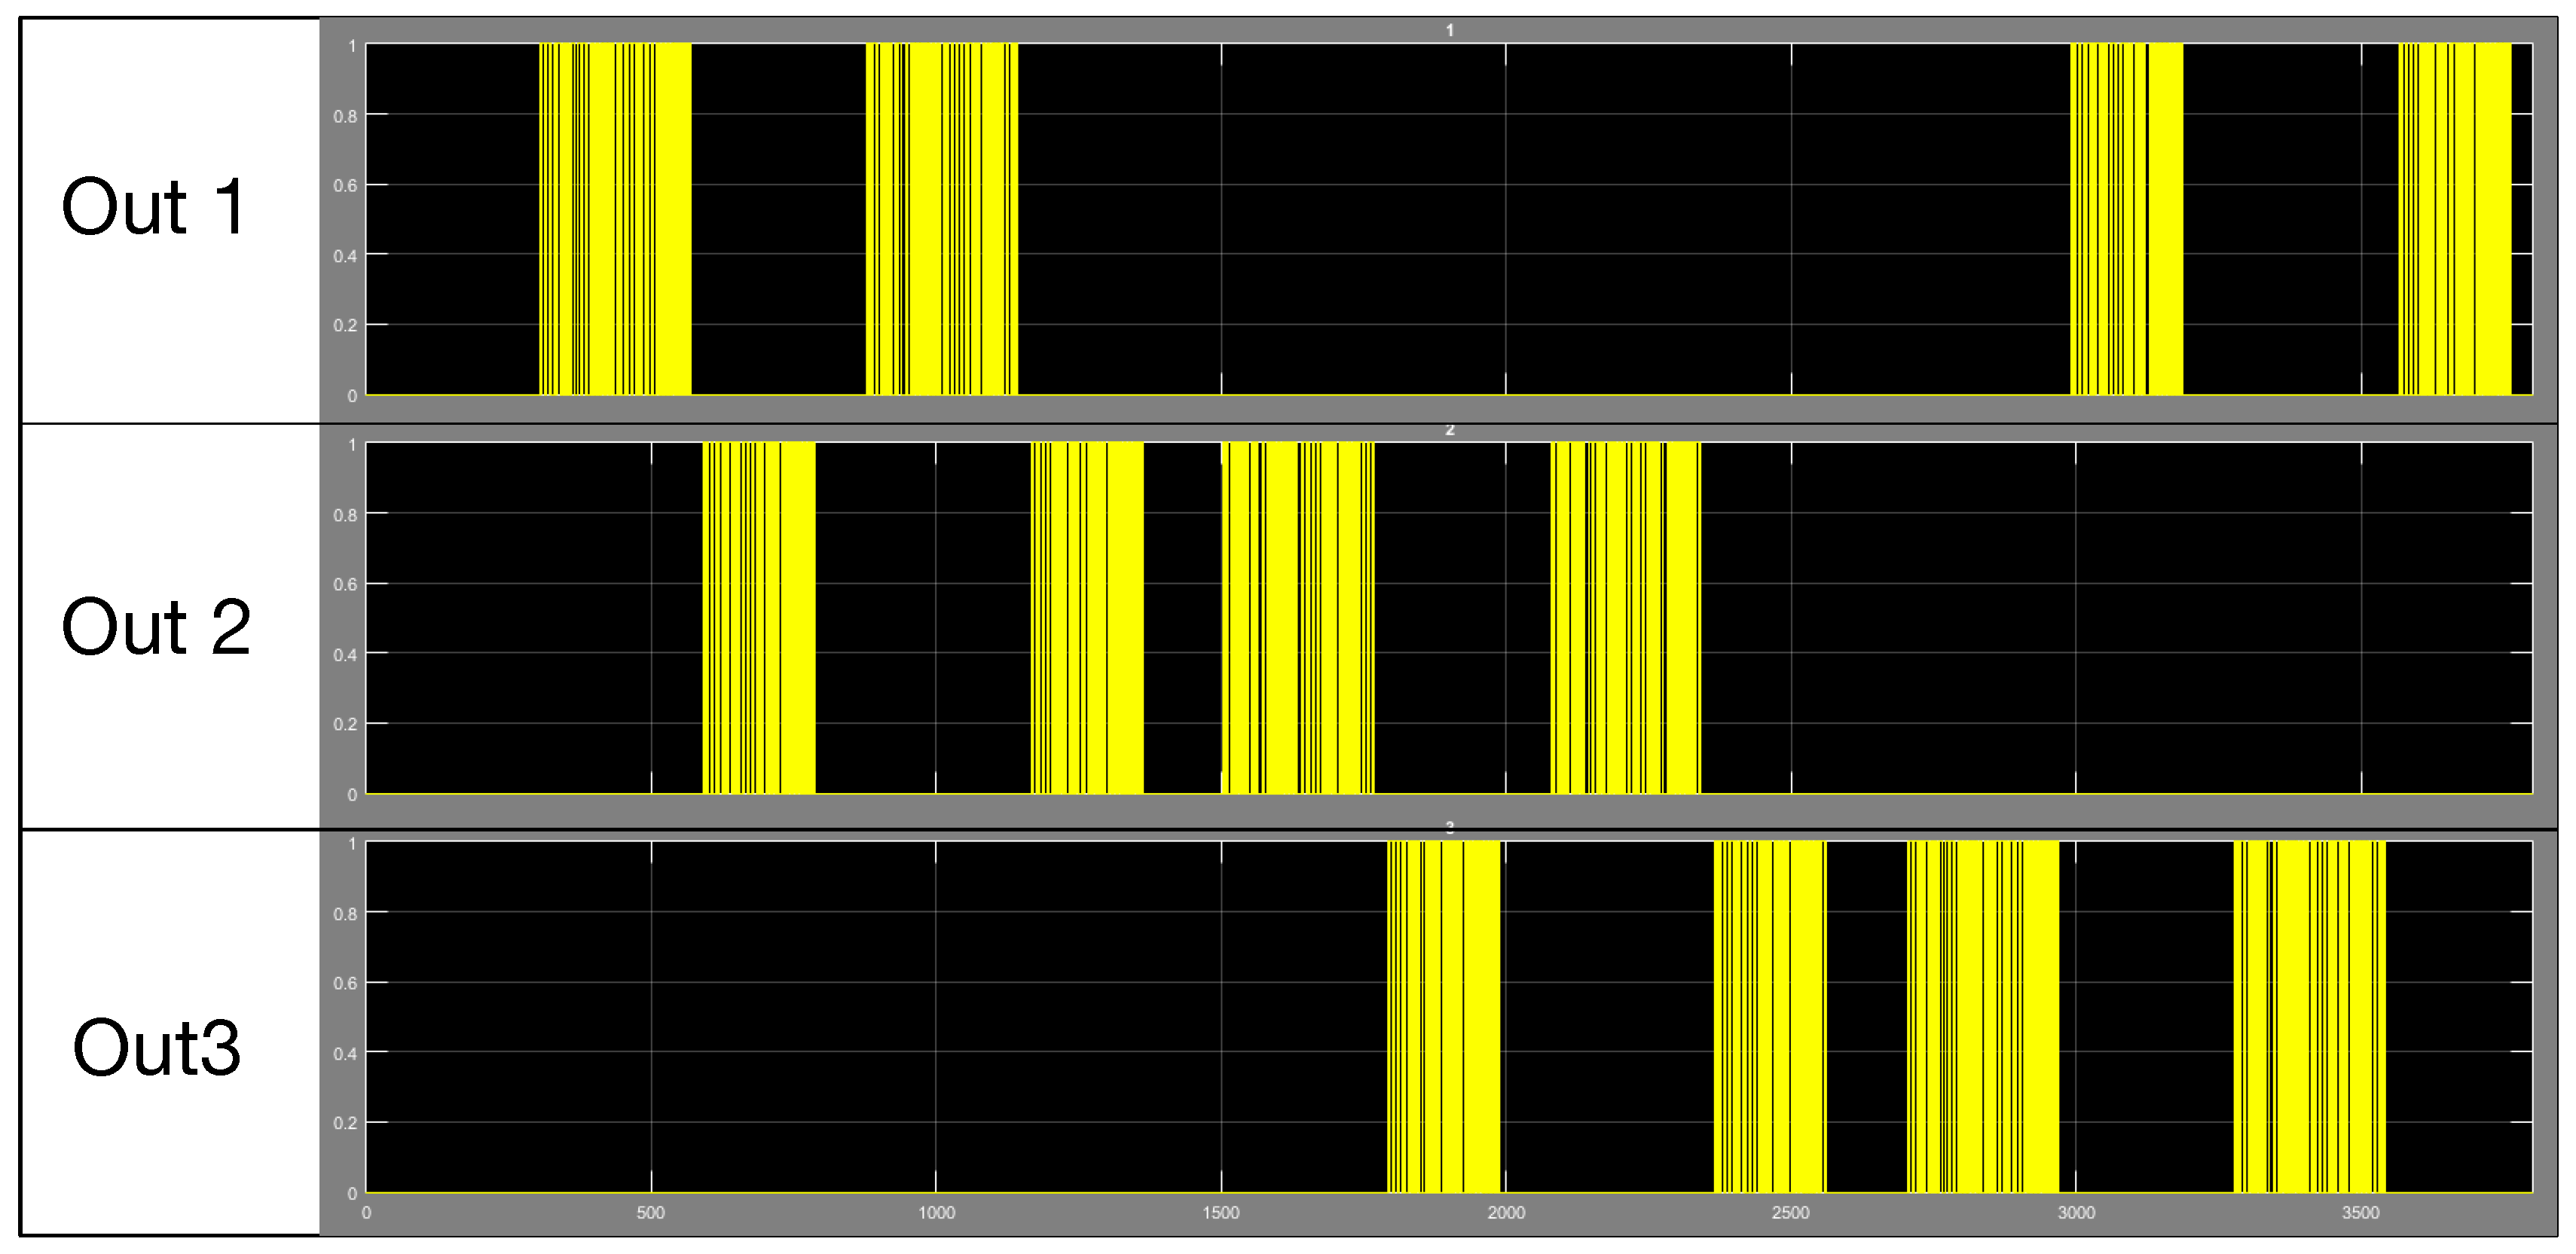
\includegraphics[width=\textwidth]{pic/Simulation_Result.pdf}
			\caption{Simulation result of mastership transfer}
			\end{figure}
		\end{column}
	
		\begin{column}{0.5\textwidth}
			We have tested the following functions:
			\begin{itemize}
			\setlength{\itemsep}{10pt}
			\item Clock signal 
			\item Mastership transfer
			\item Traffic memory
			\item Data transfer
			\item Base period
			\item ...
			\end{itemize}
		\end{column}
	\end{columns}
\end{frame}

\subsection{Code generation}

%\begin{frame}{Code generation}
%Simulink HDL Coder can generate HDL codes from Simulink models, and Stateflow charts. Generated VHDL code will be finally translated into electronic circuits. Limited by the circuit structures, not all features are supported, so there are many constraints. 
%\end{frame}


%\begin{frame}{Data staring}
%\begin{columns}[T]
%\column[c]{0.3\textwidth}
%\centering
%\begin{figure}
%	\includegraphics[width=0.9\textwidth]{pic/Data_store_memory.png}
%	\caption{Data store memory}
%\end{figure}
%
%
%\column[c]{0.7\textwidth}
%\begin{itemize}
%	\item It defines a named shared data store.
%	\item The only built in approach to share data between Charts.
%	\item Not support by HDL Coder.
%\end{itemize}
%\end{columns}
%
%\vspace{5pt}
%
%\begin{block}{Solution}
%The only way to transmit data between charts is toward input and output ports. Developers must take this into account at the beginning of design.
%\end{block}
%\end{frame}
%

%\begin{frame}{Constrains}
%	
%\begin{block}{Events usage}
%	As an Event-Driven System, the Events plays an important role in Stateflow.\\
%	You should use change of variables to take the place of the event.
%\end{block}
%
%\begin{block}{Circling number}
%	Loops in VHDL are unrolled in its corresponding hardware circuit.\\
%	Circling numbers are limited.\\
%	Can not be a variable.
%\end{block}
%
%\end{frame}


\begin{frame}{Constrains}
	After the model functions have been verified. We translated the model into VHDL codes. Limited by the circuit structure,
	some functions of formal model are not supported in circuit:
	\vspace{10pt}
	\begin{enumerate}
		\item Do not call functions recursively.
		\item Circling numbers can not be variable.
		\item Do not use pointer and address operation.
		\item Do not use events.
		\item Use no history junctions in states with parallel (AND) decomposition.
		\item Do not use Enumerated data, Simulink functions and so on.
	\end{enumerate}
\end{frame}


\begin{frame}{Technology schematic}
	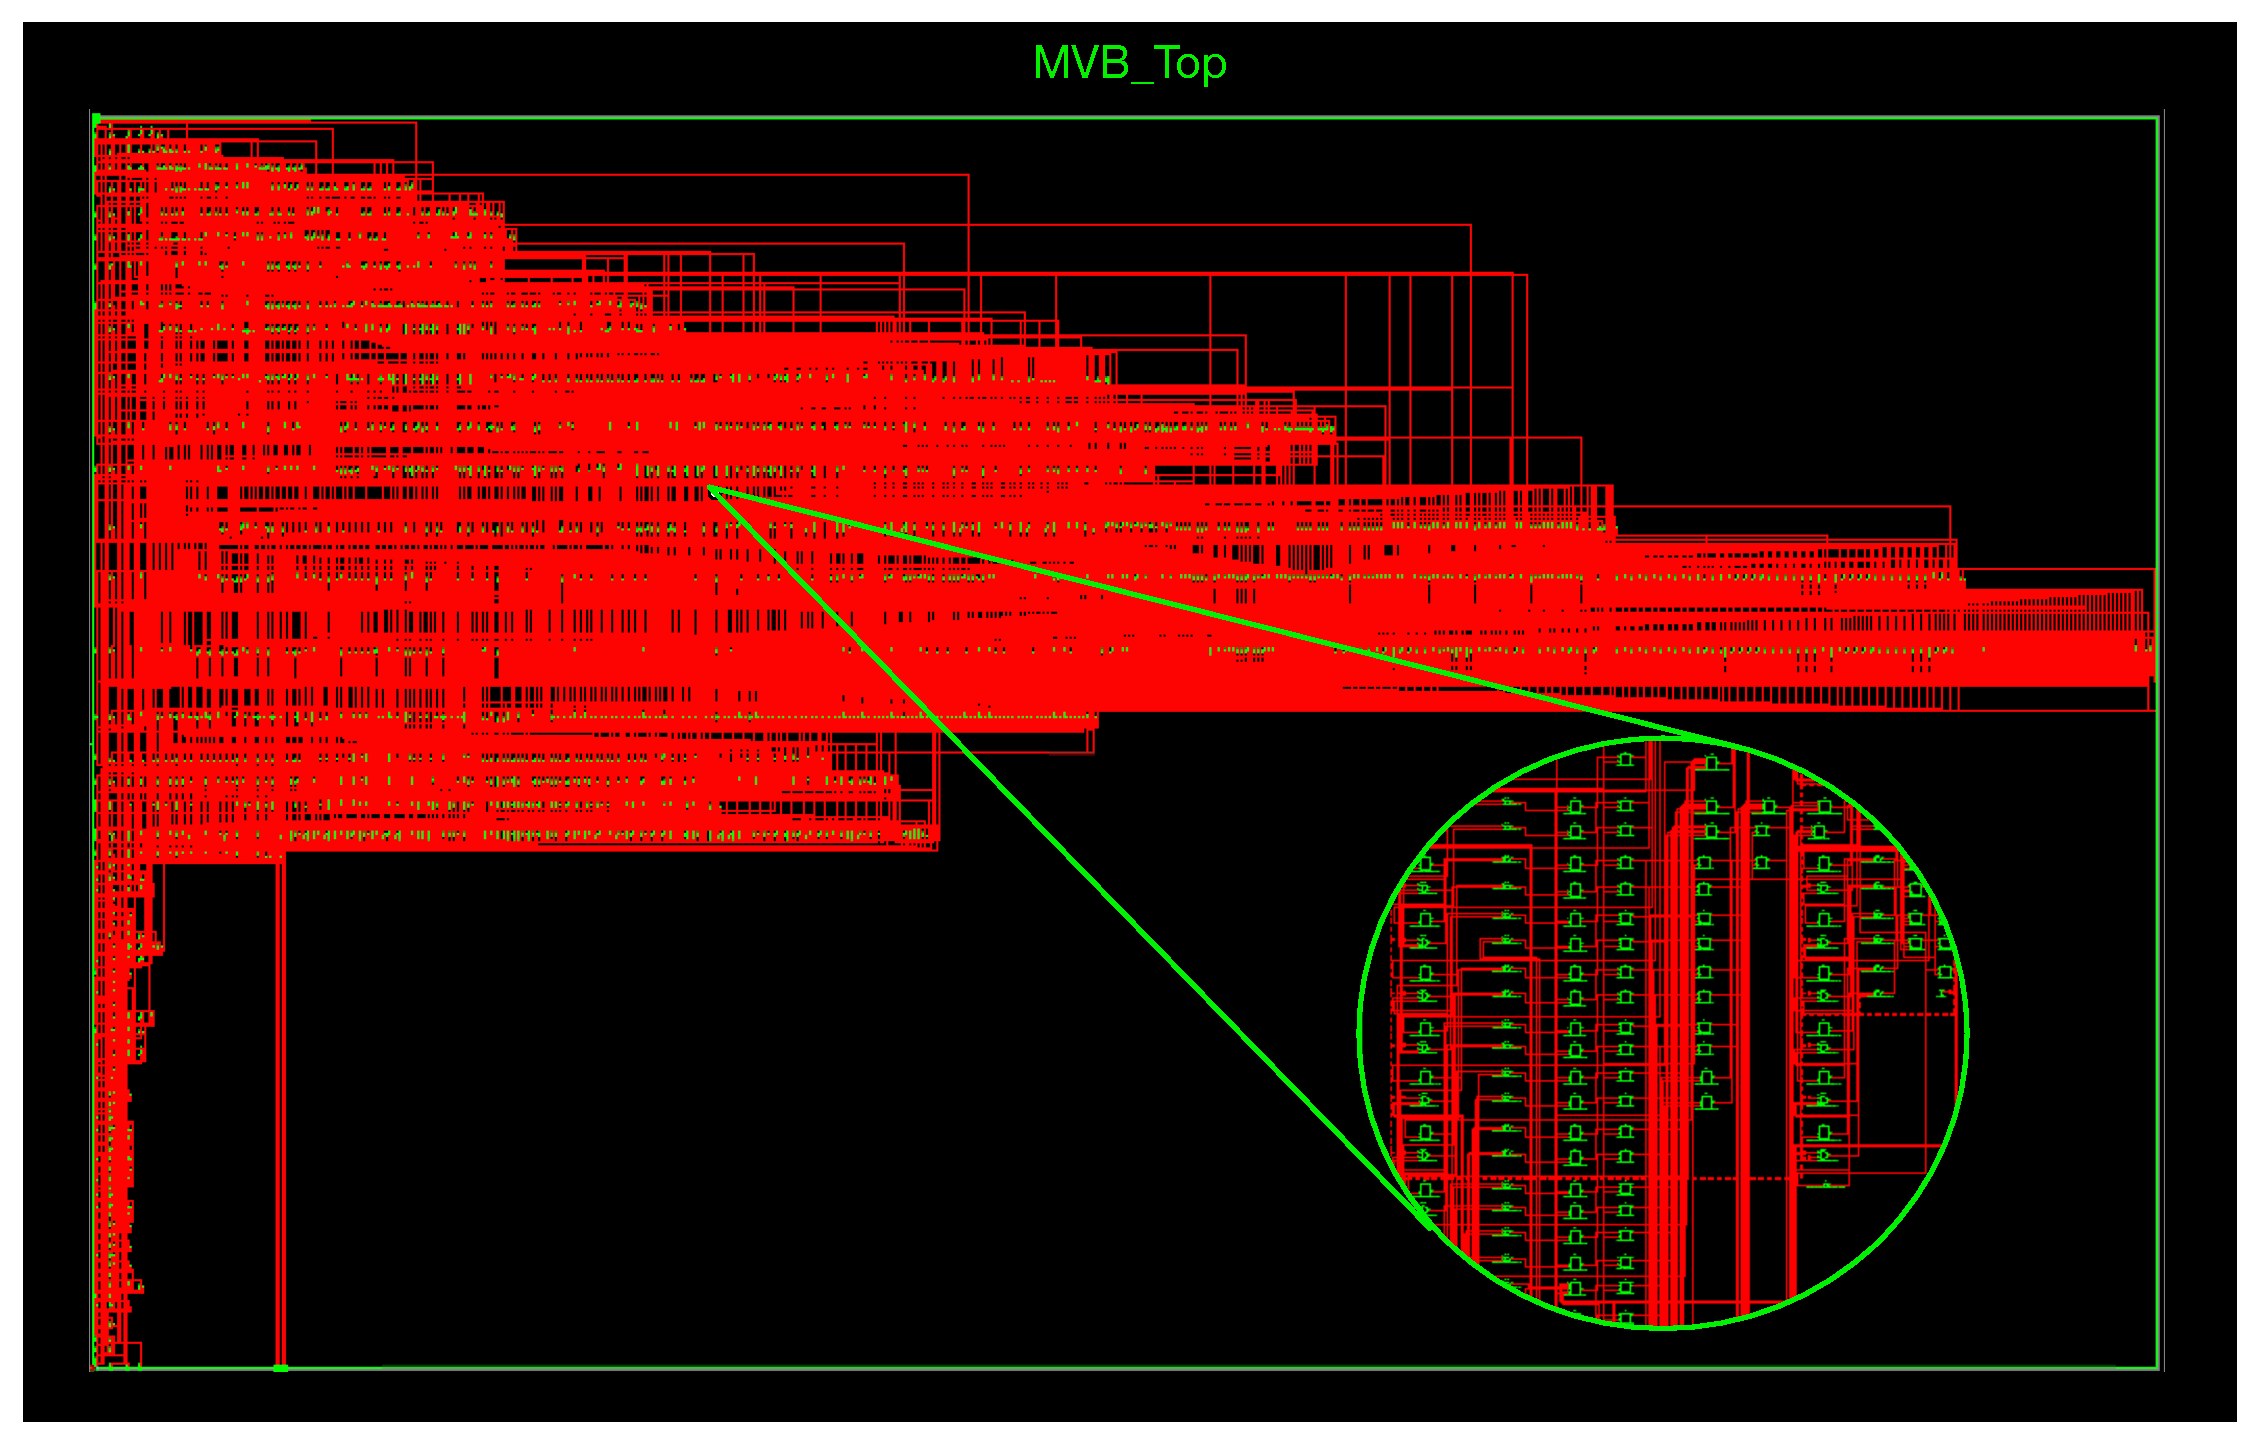
\includegraphics[width=\textwidth]{pic/TechnologySchematic.pdf}
\end{frame}




\section{Conclusion}
\begin{frame}{Conclusion}

\begin{block}{Summary}
We developed a complete MVB device with the novel formal modeling method. 

Our work provides a novel method and a different vision for numeric circuit design. 

Although this model based methodology would result in a lower performance, it can enhance the work efficiency.

\end{block}

\begin{block}{Outlook}
The generated code quality is not good enough.
We will concentrate on improving the code quality. 
\end{block}

\end{frame}

\begin{frame}[c]
	\centering
	\begin{columns}
		\column{0.7\textwidth}
			{\huge \emph{{Thank  ~you!}}}\\
	\end{columns}
\end{frame}
\end{document}


